\chapter{Evaluation}

This section presents the empirical evaluation of \textsc{Carico} as a
Kubernetes scheduler, comparing it against the default industry-standard
\texttt{kube-schedulers}. I was unable to compare \textsc{Carico} against any
similar telemetric-only schedulers due to their limited number and time
constraints. For the evaluation, I use a set of common scheduling objectives
used by data canter providers~\cite{thesis}:

\textbf{Job Completion - Section \ref{sec:eval-job-completion}:}\\
Schedulers often aim to reduce the time it takes for a job or a set of jobs to
complete. In Kubernetes, Jobs are specified by a template of the Pods to be
executed, the total number of Pods to complete (\texttt{completions}) and the
maximum number of Pods running at once (\texttt{parallelism}). Job completion
time (JCT) is defined as the time between a Job object being published to the
Kubernetes API and the time when the last Pod of the Job completes. During the
experiments, I set \texttt{parallelism} to \texttt{completions} so that only
\texttt{kube-scheduler}'s decisions impact Job completion.

\textbf{Pod Completion - Section~\ref{sec:eval-pod-completion}:}\\
Another common goal is to reduce the time it takes for idividual tasks to complete.
This section investigates the distribution of Pod Completion time (PCT): the
time it takes from when a Pod starts running to when it completes. In addition,
traces of the number of concurrently running Pods on each Node during Job
execution are used to explain the PCTs.

\textbf{Resource Utilisation - Section~\ref{sec:eval-util}:}\\
Since resources are expensive, data canters aim to ensure that resources are
well utilised with efficient placements. Over-utilisation can result in large
amounts of resource thrashing, which wastes resources and hurts a data canters
profitability. As \textsc{Carico} currently only uses CPU and memory metrics
for scheduling, only the utilisation of those resources are measured during the
execution of Jobs.

\textbf{Workload Heterogeneity - Section~\ref{sec:eval-hetero}:}\\
As outlined in \ref{sec:background-datacenters}, data canters must handle
workloads with different characteristics, such as, resource usage and running
times. This section evaluates \textsc{Carico} performance with multiple Jobs
with different characteristics.

\textbf{Workload Isolation - Section~\ref{sec:eval-isolation}:}\\
Data canters have to deal with jobs with different QoS requirements. One of
these requirements is workload isolation: whether the execution of one Job will
interfere with the execution of another, impacting a user's experience. This
experiment measures the impact on a scheduling decisions on the response latency
of a server running in the cluster.

\textbf{Overhead - Section~\ref{sec:eval-overhead}:}\\
Due to the limited number of resources that need to be shared between users,
schedulers must mitigate their overhead. A lower overhead frees up more
resources for users and providers can achieve higher profits margins. This
experiment measures the overhead incurred from running the DaemonSet of
\textsc{Carico} Pods.

To ensure a fair comparison between \textsc{Carico} (telemetric-only scheduler)
and \texttt{kube-scheduler} (resource description-based scheduler), I use a
range of resource requests with \texttt{kube-scheduler} to highlight how much
the performance can vary with different resource request.

\section{Evaluation Setup}
These experiments ran on a Kubernetes cluster containing 20 virtual machines
(VMs) running on the Xen hypervisor. One of the machines is used as the master
Node, and the rest are worker Nodes. The master Node contains all the Pods in
the control plane, and during the evaluation of \textsc{Carico}, it contains the \textsc{Carico}
Scheduler and Aggregation Server. Each VM advertises four Intel Xeon Gold 6142
CPUs \@ 2.60GHz with 8 GB of RAM running Ubuntu 24.04.2 LTS. Each CPU has a
single core with hyper-threading disabled. When running \texttt{kubectl describe
nodes}, each Node advertises $4000$ milliCPU seconds and 8GB of RAM.

During the evaluation, I use a Prometheus deployment \cite{} to collect various
statistics, such as running Pod count, resource utilisation and Kubernetes
object completions.

%
% For any practical projects, you should almost certainly have some kind
% of evaluation, and it's often useful to separate this out into its own
% chapter.

\section{Experimental Workloads}
During the experiments I used very short-lived workloads; workloads that take
less than a minute to complete. While data canters can expect to receive
longer-running workloads, using them in the evaluation was not feasible due to
the need to run experiments multiple times and limited time. Short-lived tasks
can still provide valuable insights into the performance of a scheduler as their
short completion time makes the impact of poor scheduling decisions more
significant and easier to observe.

During this evaluation, I used two types of workloads:
\begin{enumerate}
    \item \texttt{pi-2000}: A short-lived CPU-focused workload where a Pod
        computes the value of $\pi$ to 2000 decimal points.
    \item \texttt{sklearn}: A longer-running workload with a larger memory
        footprint. This Pod executes a script which uses
        \texttt{sklearn} which trains a small neural network classifier ($512$
        features, $16$ classes, $8$ hidden layers each containing $1024$
        neurons) on 5000 randomly generated samples before running inference on
        another set of 5000 randomly generated samples.
\end{enumerate}
Investigating metrics when running \texttt{pi-2000} and \texttt{sklearn} Jobs
separately demonstrates how \textsc{Carico} handles opposing resource usage
characteristics (CPU-focused vs memory-focused). Furthermore, when executing
both these Jobs concurrently, the difference in runtime helps investigate how
\textsc{Carico} also handles workloads with different running times.

% In this experiment, I use a Job that specifies Pods that performed a small ML
% workload. This workload uses a significant amount of memory, which unlike CPU,
% must be carefully handled. If we increase the number of processes on a
% fully-utilised CPU, it only results in each process having a smaller portion of
% CPU time and degrading its performance. On the other hand, memory is less
% forgiving as once memory runs out, the kernel begins OOM killing processes. This
% be detrimental to Job Completion, as terminated Pods results in wasted
% computations.
%

\section{Job Completion}
\label{sec:eval-job-completion}

% \begin{table}[ht!]
% \centering
    % \begin{tabular}{|l|r|c|c|c|c|c|}
    % \hline
    % \textbf{Scheduler} & \textbf{Requested} & \multicolumn{5}{c|}{\textbf{Job Completion (s)}} \\
    % \cline{2-7}
    % &  \textbf{CPU} & \textbf{100 Pods} & \textbf{250 Pods} & \textbf{500 Pods} & \textbf{750 Pods} & \textbf{1000 Pods} \\
    % \hline
    % \texttt{kube-scheduler} & 100m & 15.7 $\pm$ 0.6 & 31.7 $\pm$ 2.1 & 56 $\pm$ 1.7 & 84.7 $\pm$
        % 0.6 & 112 $\pm$ 0.0 \\
    % \texttt{kube-scheduler} & 200m & 15.7 $\pm$ 0.7 & 30.7 $\pm$ 0.6 & 55 $\pm$ 1 & 79 $\pm$ 0.0
        % & 103 $\pm$ 1 \\
    % \texttt{kube-scheduler} & 500m & 15.7 $\pm$ 1.2 & 32 $\pm$ 2.6 & 57.7 $\pm$ 0.6 & 81 $\pm$ 2
        % & 104 $\pm$ 2.1 \\
    % \texttt{kube-scheduler} & 1000m & 21 $\pm$ 2.0 & 54.7 $\pm$ 0.6 & 96 $\pm$ 2.6 & 133 $\pm$
        % 0.6 & 175 $\pm$ 1 \\
    % \textsc{Carico} &  & 20.3 $\pm$ 0.6 & 35.3 $\pm$ 0.6 & 60.3 $\pm$ 2.5 & 89 $\pm$ 2 &
        % 109$\pm$ 1 \\
    % \hline
    % \end{tabular}
    % \caption{Job Completion of Job deployments with different Pod counts. Each
    % Pod executed \texttt{bpi(2000)}. For the default scheduler, the requested
    % resources are also given}
    % \label{tab:pi-2000-throughput}
% \end{table}
%

\begin{figure}[ht!]
    \centering
    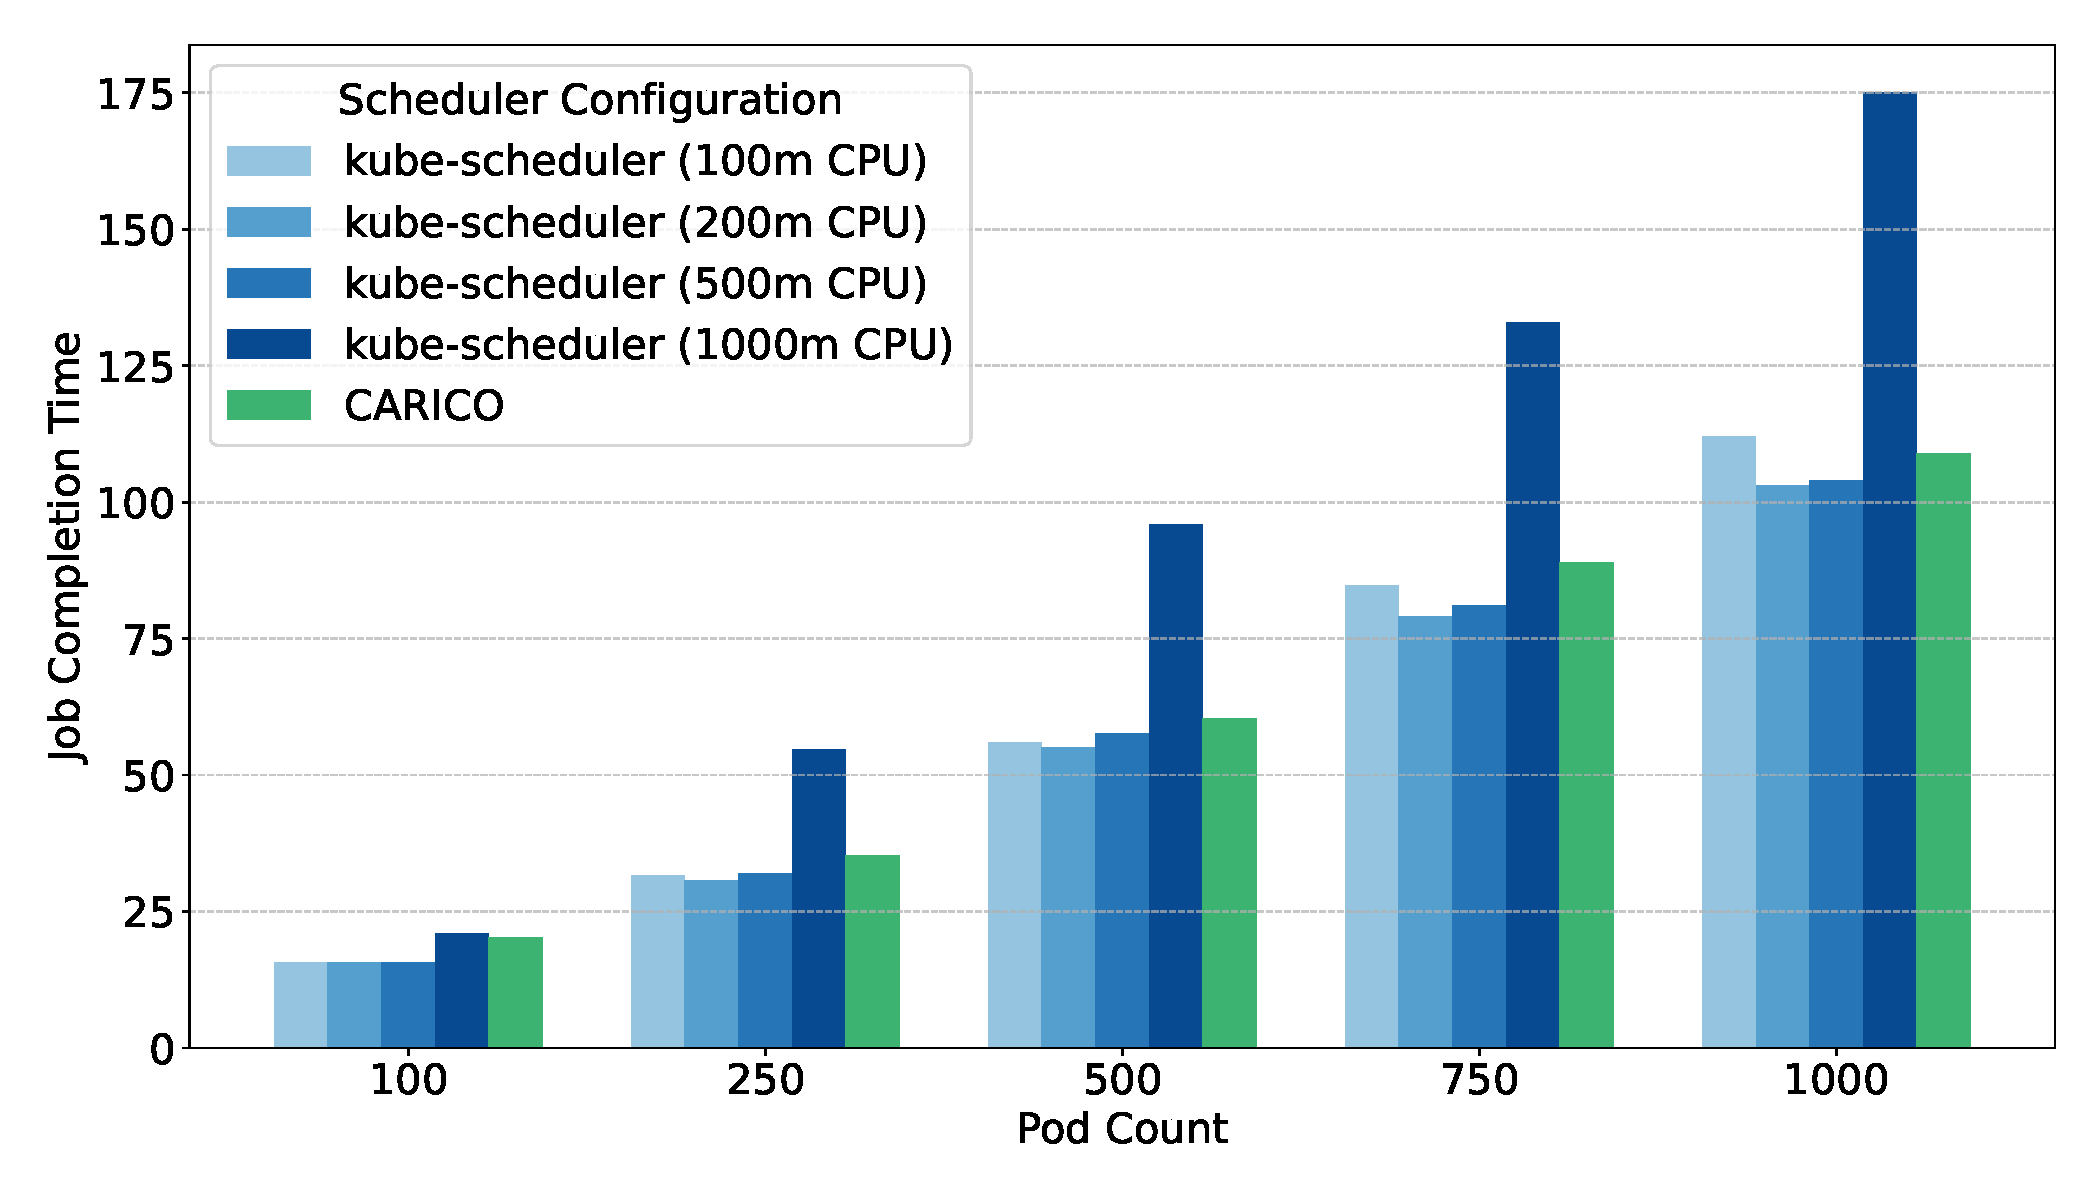
\includegraphics[width=\textwidth]{images/pi-job-completion.pdf}
    \caption{The Job completion of \texttt{pi-2000} Jobs with different Pod
    counts. The requested resources are given when using \texttt{kube-scheduler}}
    \label{fig:pi-2000-throughput}
\end{figure}

Figure \ref{fig:pi-2000-throughput} demonstrates the JCT of
\texttt{pi-2000} with different Pod counts. We can observe that \textsc{Carico}
is able to consistently achieve comparable JCT (within $\approx$
10\% of the optimal run with \texttt{kube-scheduler}) without any prior
knowledge of a Pod's resource usage. On the other hand, incorrect Pod requests
can result in $\approx$ 80\% increase in Job completion when using
\texttt{kube-scheduler}.

% \begin{table}[ht!]
% \centering
    % \begin{tabular}{|l|r|r|c|c|}
    % \hline
    % \textbf{Scheduler} & \multicolumn{2}{c|}{\textbf{Requested}} &
        % \multicolumn{2}{c|}{\textbf{Job Completion (s)}} \\ \cline{2-5}
    % &  \textbf{CPU} & \textbf{Memory} & \textbf{100 Pods} & \textbf{200 Pods} \\
    % \hline
        % \texttt{kube-scheduler} & 200m & 750Mi & 144.3 $\pm$ 0.6 & 362 $\pm$ 20.4\\
        % \textsc{Carico} &  &  & 189 $\pm$ 4.36 & 353.3 $\pm$ 12.7 \\
    % \hline
    % \end{tabular}
    % \caption{Job Completion of Job deployments with different Pod counts. Each
    % Pod executed a small ML workload. For the default scheduler, the requested
    % resources are also given}
    % \label{tab:ml-throughput}
% \end{table}

\begin{figure}[ht!]
    \centering
    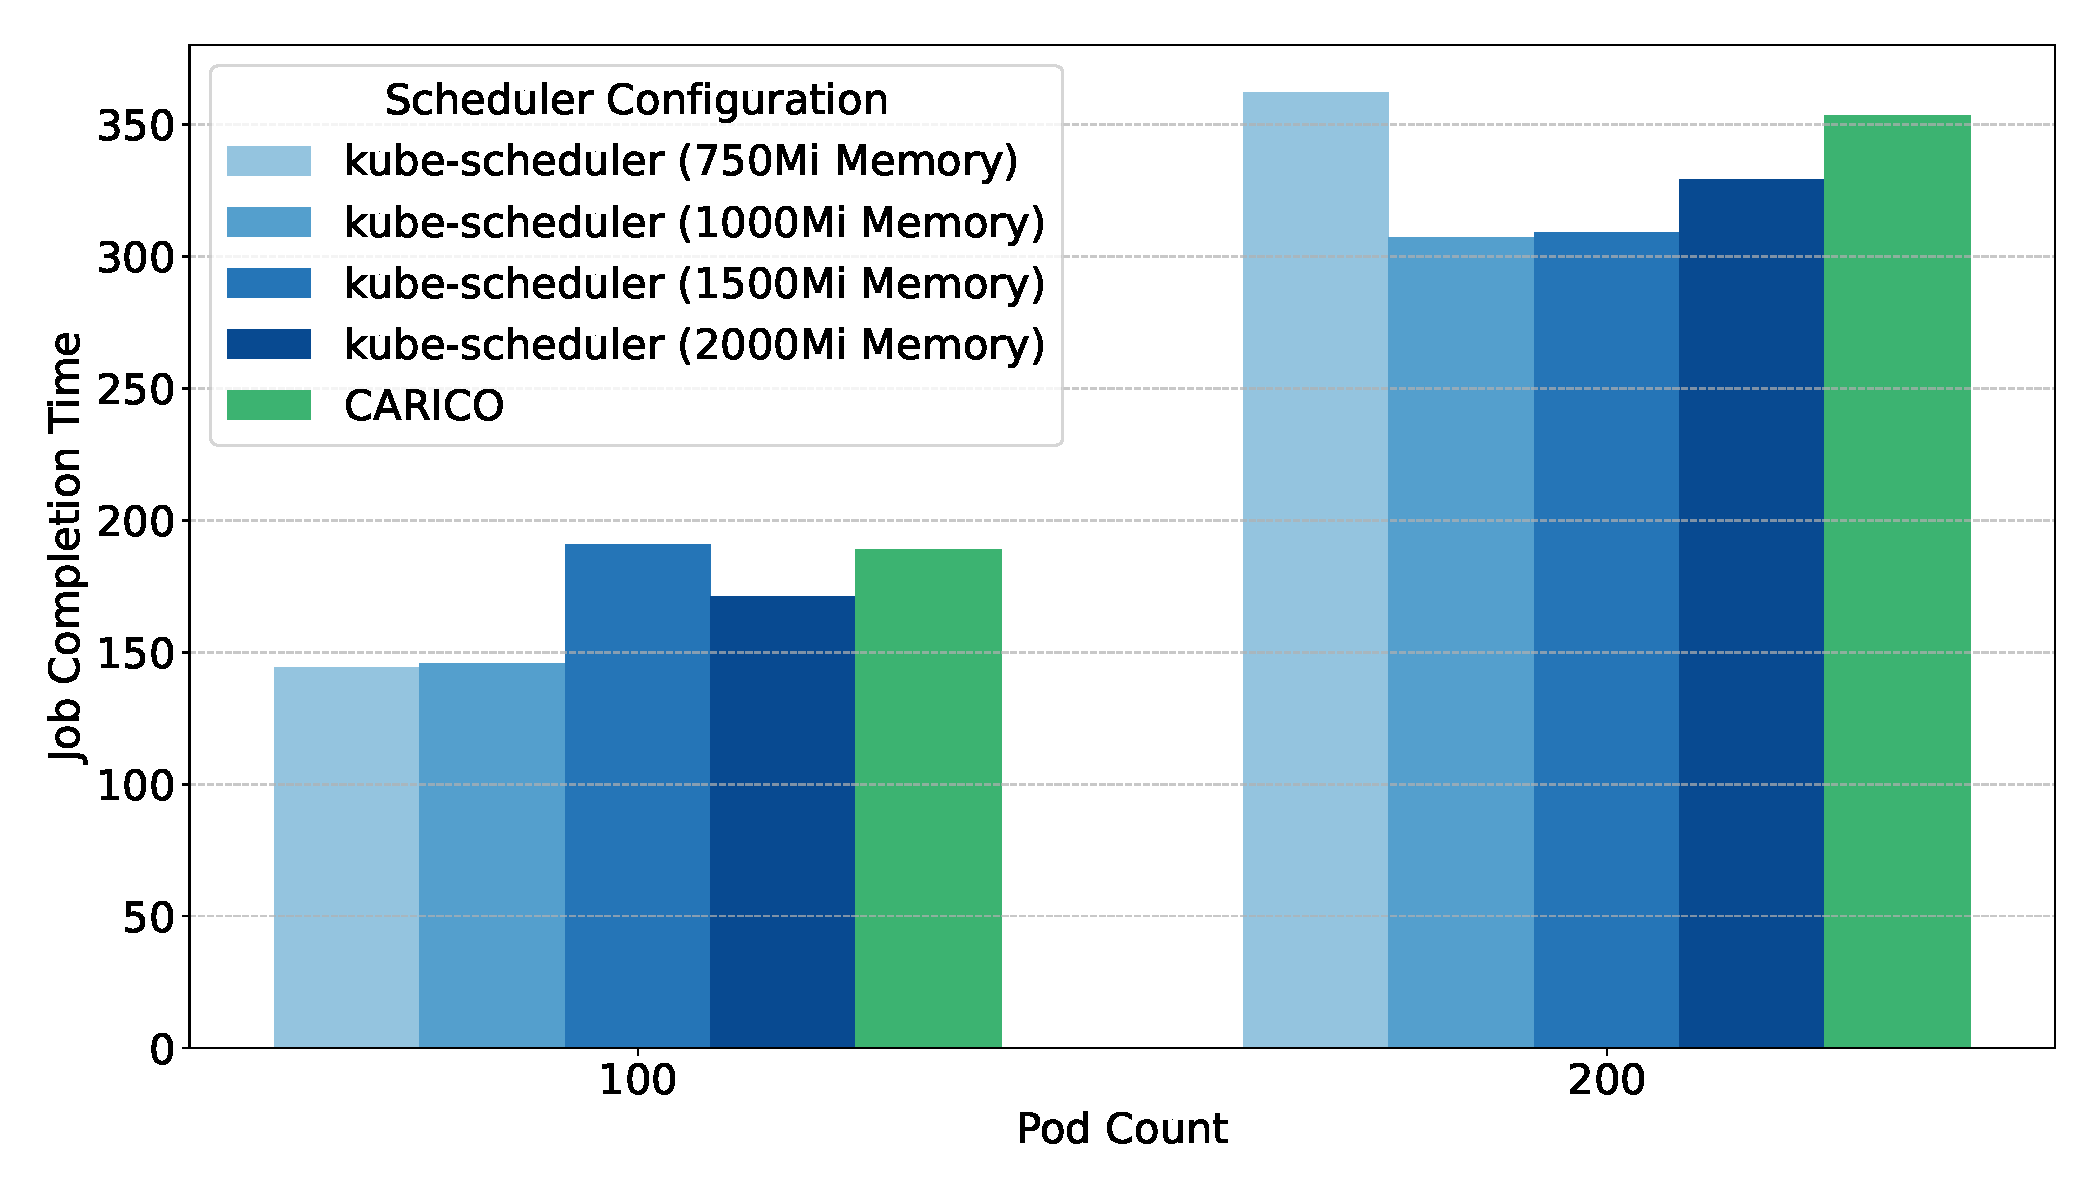
\includegraphics[width=\textwidth]{images/ml-job-completion.pdf}
    \caption{The Job completion of \texttt{sklearn} Jobs with different Pod
    counts. The requested resources are given when using
    \texttt{kube-scheduler}}
    \label{fig:ml-throughput}
\end{figure}

Figure \ref{fig:ml-throughput} presents the JCT of \texttt{sklearn}
Jobs. Similarly \textsc{Carico} is able to achieves comparable JCTs using only
telemetric data. Similarly, we can also observe how JCT varies with different
resource requests. More importantly, underestimating memory usage can result in
Nodes running out of memory and their kernel Out-Of-Memory (OOM) killing running Pods.
This can result in Jobs failing to complete and is the reason for why we do not
present the JCT for runs requesting less than 750Mi bytes of memory.

\section{Pod Completion}
\label{sec:eval-pod-completion}
In this section, I compare the individual Pod Completion times (PCT) from the
traces of different Job executions.

\begin{table}[h!]
\centering
    \begin{tabular}{|l|r|c|c|c|c|c|c|c|}
    \hline
        \bfseries Scheduler & \bfseries CPU Request & \bfseries Mean & \bfseries Std. &
        \bfseries Min. & \bfseries 25\% & \bfseries Median & \bfseries 75\% & \bfseries Max. \\
    \hline
        \texttt{kube-scheduler} & 100m & 47.43 & 14.59 & 7.00 & 39.00 & 52.00 & 57.00 & 73.00
        \\
        \texttt{kube-scheduler} & 500m & 9.55 & 1.49 & 5.00 & 9.00 & 10.00 & 10.00 & 14.00
        \\
        \textsc{Carico} & & 7.69 & 0.99 & 5.00 & 7.00 & 8.00 & 8.00 & 11.00 \\
    \hline
    \end{tabular}
    \caption{PCT of a trace when executing a \texttt{pi-2000} Job
    with 1000 Pods under different schedulers.}
    \label{tab:cpu-pod-completions}
\end{table}

Table \ref{tab:cpu-pod-completions} demonstrates \textsc{Carico} ability to
achieve a tight Pod completion distribution with 75\% of Pods completing in less
than 8 seconds. In contrast, underestimating resource requests with 100
milliCPU, the distribution of PCT becomes tail-heavy with 50\% of Pods taking
longer than 52 seconds to complete and a maximum completion time of 73 seconds.
Even when using the optimal and more conservative resource request of 500
milliCPU, comparing its PCT with \textsc{Carico} gives 25\% higher mean with
50\% more variance.

\begin{figure}[ht!]
    \centering
    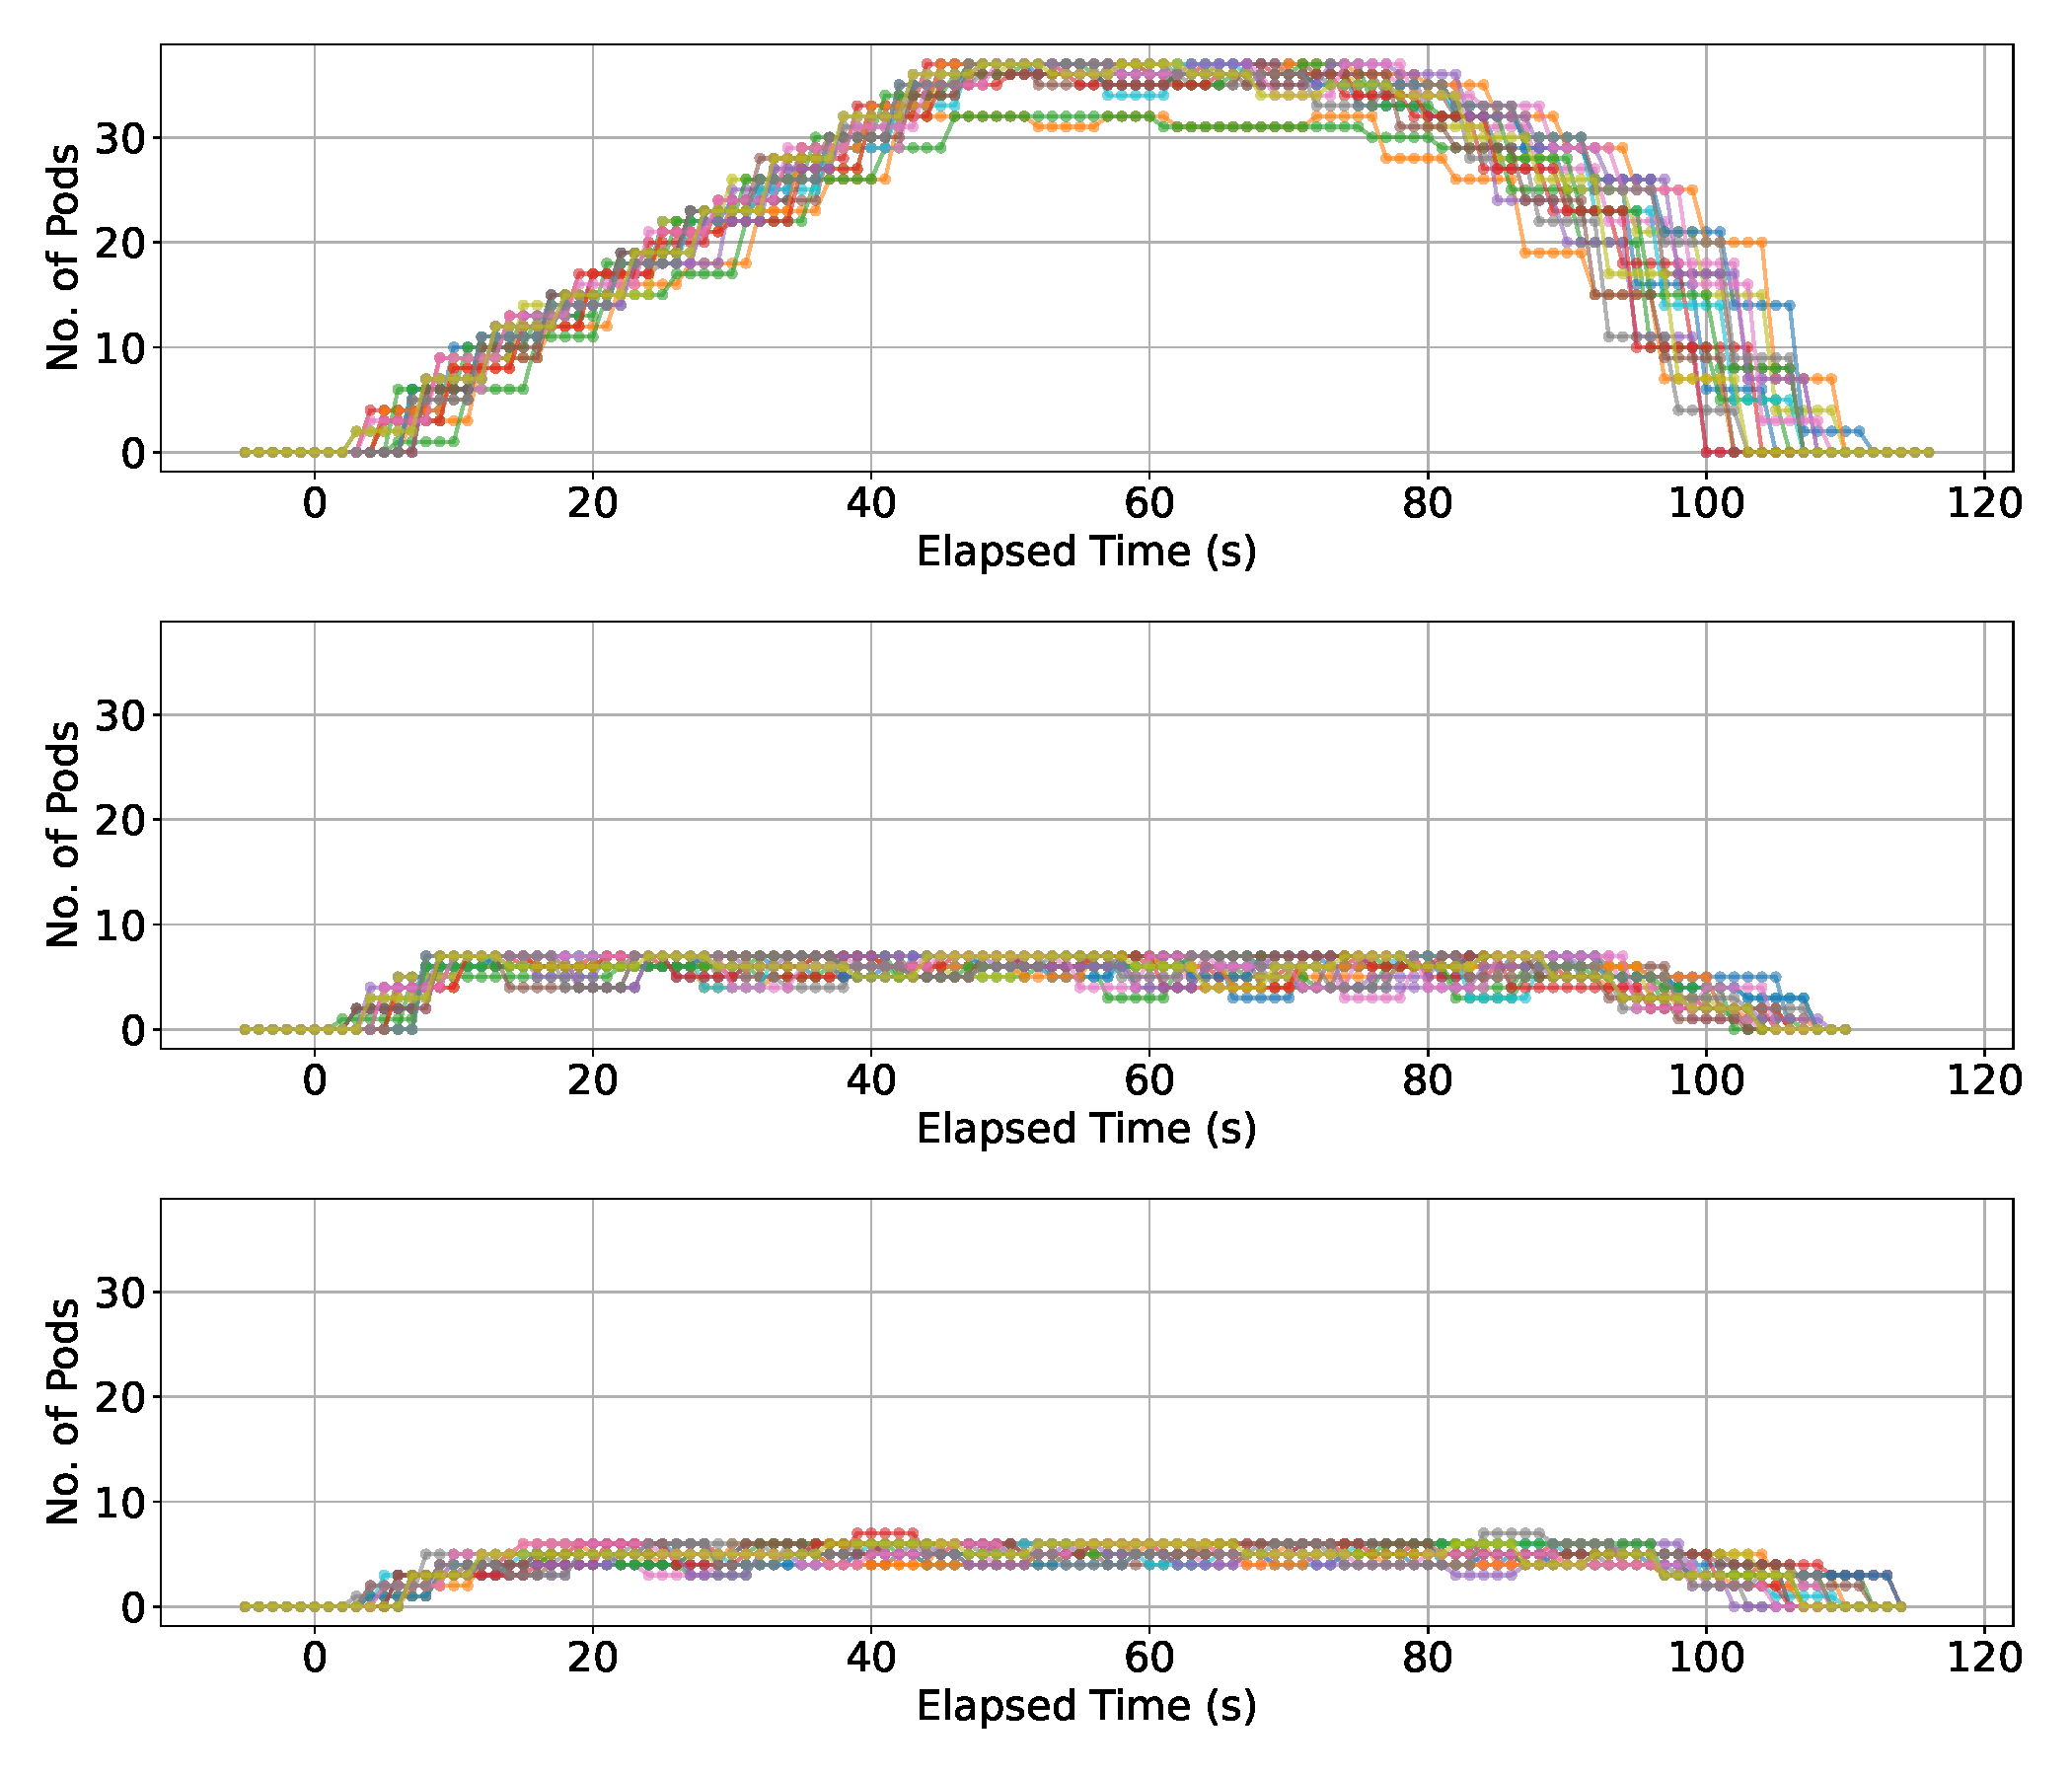
\includegraphics[width=\textwidth]{images/pi-running-pods.pdf}
    \caption{The number of \texttt{pi-2000} Pods running on a Node during the
    execution of a Job with 1000 Pods. Top: \texttt{kube-scheduler} (100m).
    Middle: \texttt{kube-scheduler} (500m). Bottom: \textsc{Carico}}
    \label{fig:pi-2000-1000x-pod-running}
\end{figure}

Figure \ref{fig:pi-2000-1000x-pod-running} gives the running Pod count of Nodes
during the runs used in Table \ref{tab:cpu-pod-completions}. Underestimating the
resource request allows \texttt{kube-scheduler} to pack more Pods on a Node at
once. This results in higher resource contention as more Pods have to share
their time on the CPU and take longer to finish their computation. Conversely,
a conservative request means \texttt{kube-scheduler} packs
fewer Pods. Each Pod a large share of CPU time and can complete faster.
\textsc{Carico} achieves a similar result to the optimal conservative request,
as Nodes detect the CPU is at capacity once there is always at least one process
waiting for a CPU core. This therefore limits the number of Pods a Node can take
and ensures all Pods receive an adequate amount of CPU resources.

\begin{table}[ht!]
\centering
    \begin{tabular}{|l|r|c|c|c|c|c|c|c|}
    \hline
        \bfseries Scheduler & \bfseries \# Pods & \bfseries Mean & \bfseries Std. &
        \bfseries Min. & \bfseries 25\% & \bfseries Median & \bfseries 75\% & \bfseries Max. \\
    \hline
        \texttt{kube-scheduler} & 100 & 127.38 & 5.29 & 118 & 123.00 & 126.00 & 132.00 &
        138.00 \\
        \textsc{Carico} & 100 & 59.02 & 14.62 & 27.00 & 55.00 & 61.00 & 66.00 & 94.00 \\
        % \texttt{kube-scheduler} & 200 & 225.19 & 36.19 & 45.00 & 231.00 & 236.00 & 239.00 &
        % 244.00\\
        % \textsc{Carico} & 200 & 64.46 & 14.33 & 23.00 & 57.75 & 67.00 & 73.25 & 89.00 \\
    \hline
    \end{tabular}
    \caption{PCT of a trace when executing a \texttt{sklearn} Job
    with 100 Pods under different schedulers.}
    \label{tab:mem-pod-completions}
\end{table}

Table \ref{tab:mem-pod-completions} shows \textsc{Carico} continues to achieve a
lower average PCT when scheduling memory-centric workloads.
However, when using the lowest overestimate of memory utilisation, 750Mi bytes
of memory, \texttt{kube-scheduler} achieves tighter PCT distribution.

\begin{figure}[ht!]
    \centering
    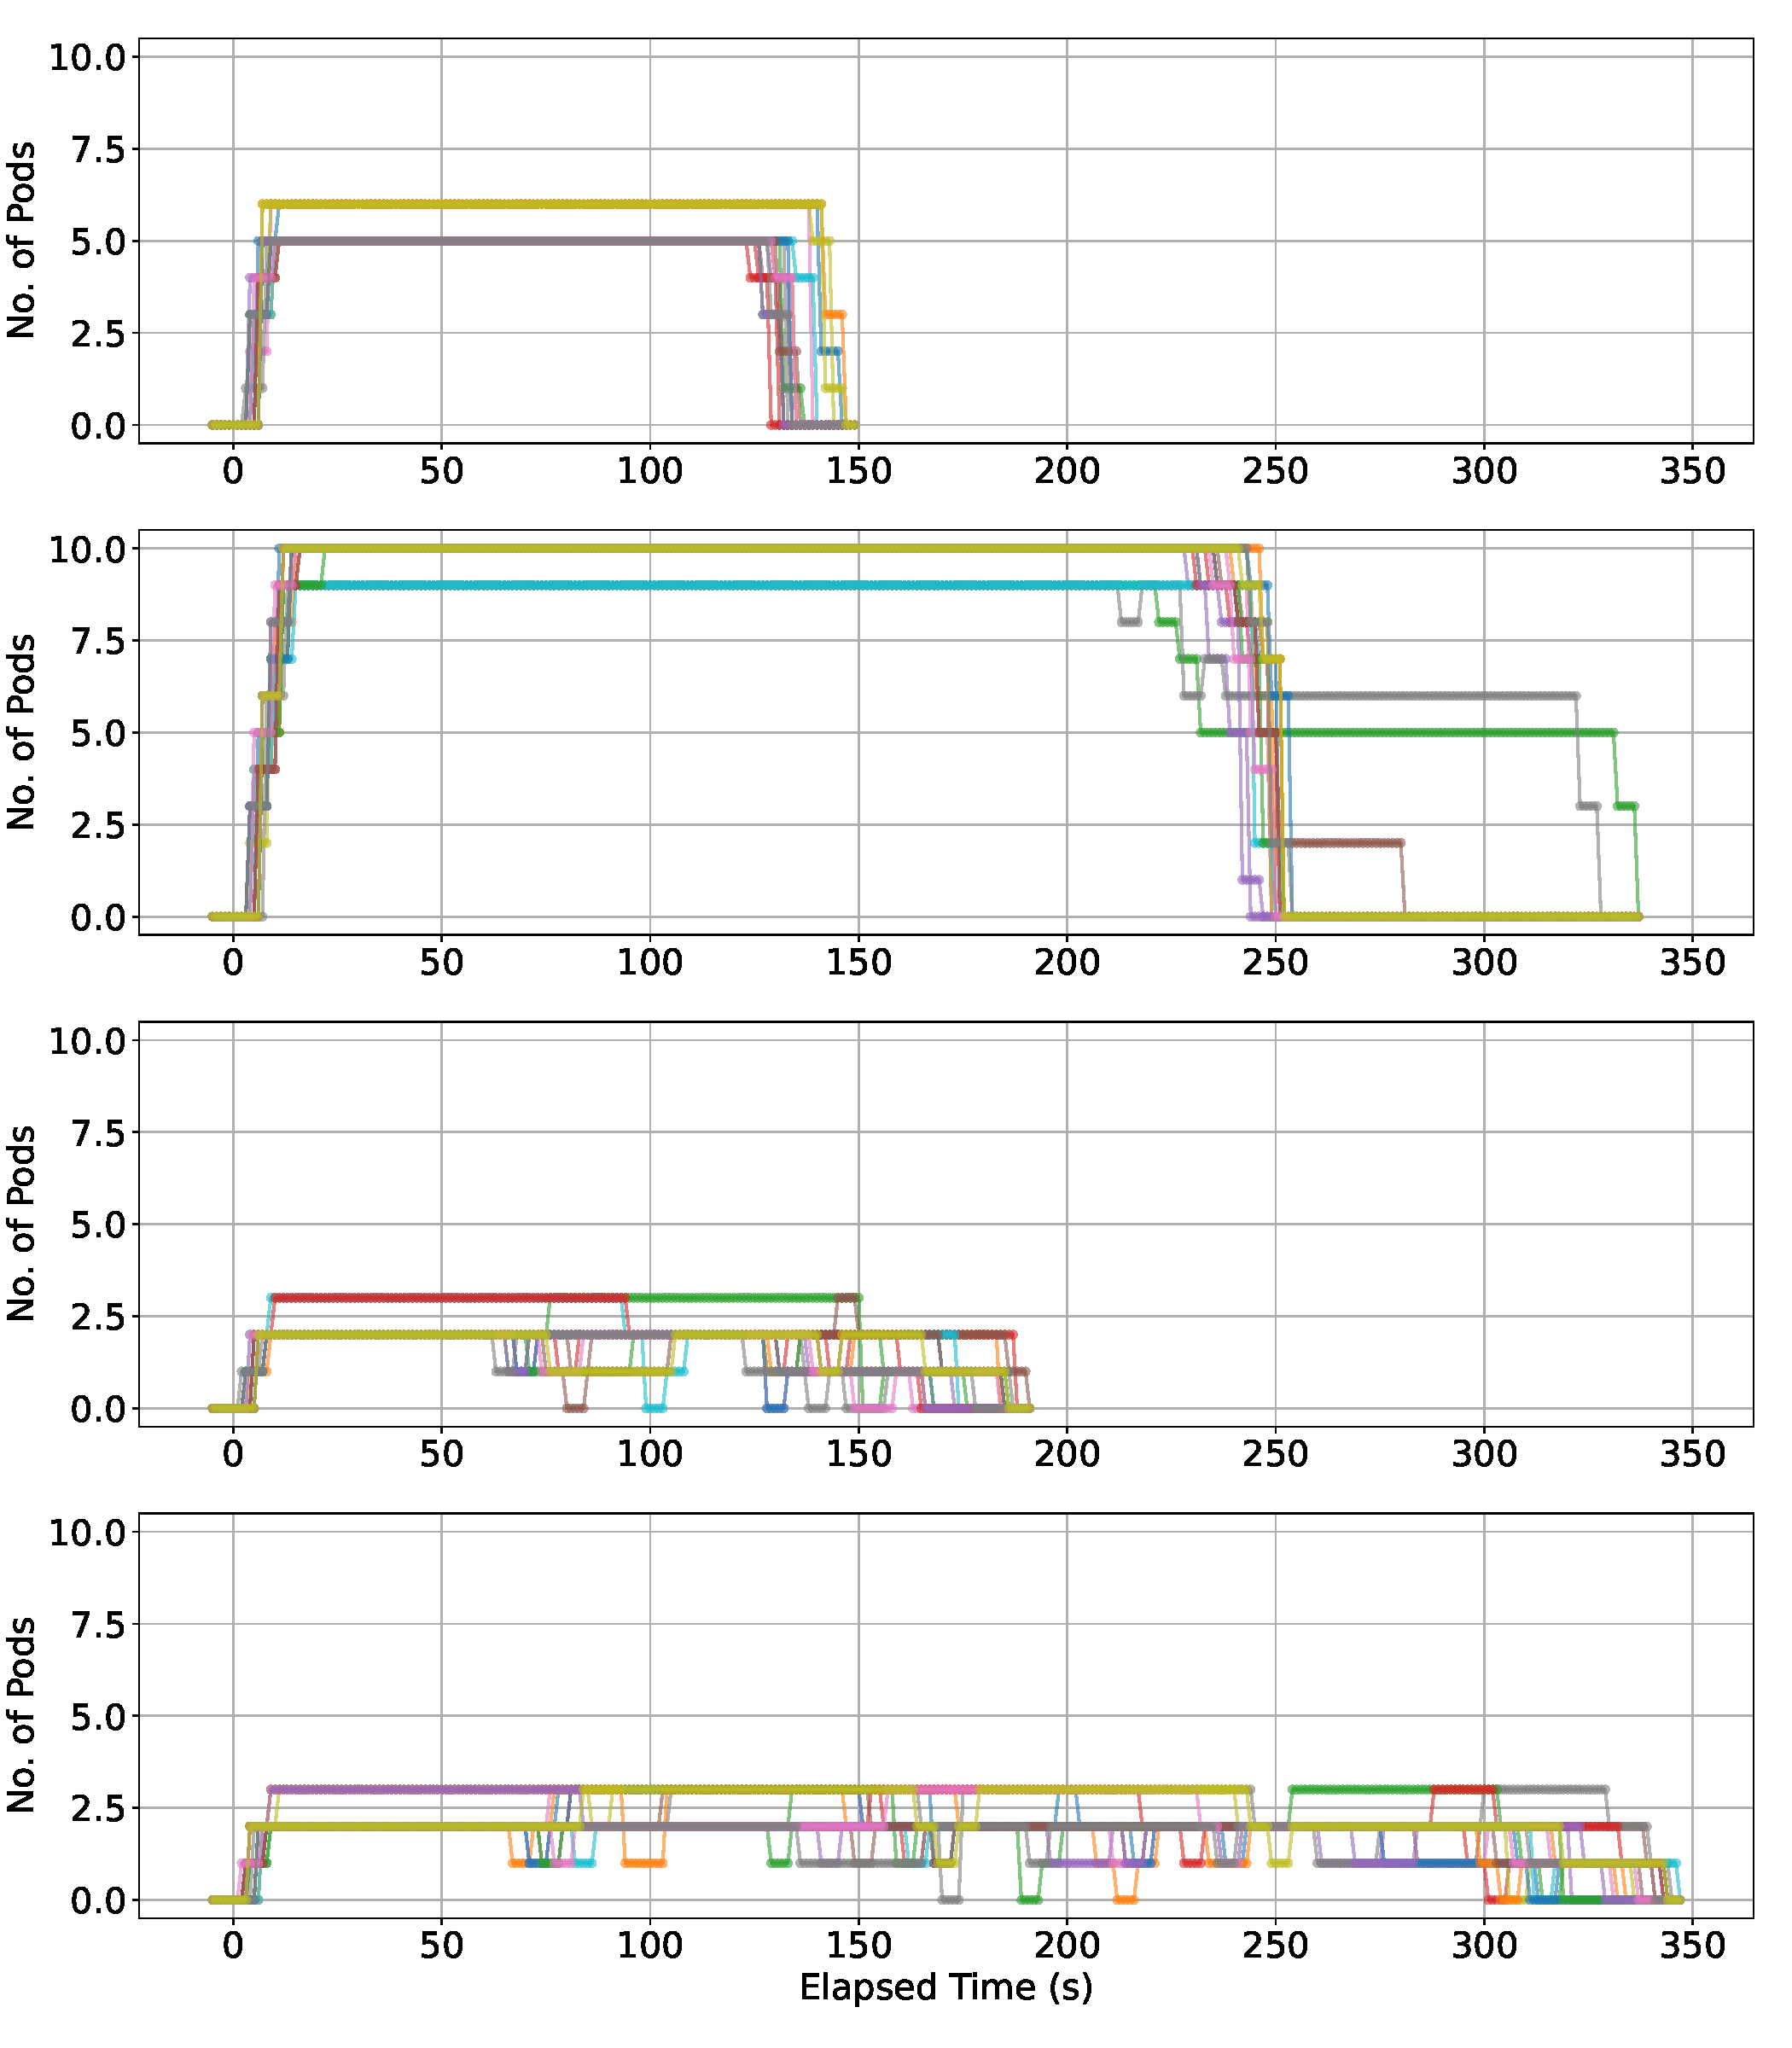
\includegraphics[width=\textwidth]{images/ml-running-pods.pdf}
    \caption{The number of \texttt{sklearn} Pods running on a Node during the
    execution of a Job with 100 Pods. Top: \texttt{kube-scheduler} (750Mi).
    Bottom: \textsc{Carico}}
    \label{fig:ml-pod-running}
\end{figure}

Like with \texttt{pi-2000}, \texttt{kube-scheduler} still allocates more Pods
onto a Node at once, resulting in higher resource contention, and thus longer
mean PCT. However, all the Pods complete around the same time resulting in a
smaller variance. With \textsc{Carico}, Nodes have fewer running Pods and so
Pods can complete faster. In addition, there's evidence of inefficiency with
\textsc{Carico}, as Nodes occasionally have no Pods running showing that. This
combined with the relationship between JCT and the number of running Pod also
explains \textsc{Carico}'s higher JCT.
%
%
% This graph also explains the longer Job completion time. Due
% to the memory request (750 Mi) and each Node's capacity (8GB),
% \texttt{kube-scheduler} is unable to allocate all the Pods in one sweep.
% However, once the Pods on the faster machines (imbalance caused by the
% hypervisor) complete, \texttt{kube-scheduler}'s greedy nature causes it to
% allocate all the remaining Pods to those machines. The long running time of the
% \texttt{sklearn} Pods combined with the resource contention from allocating the
% remaining Pods to a small number of machines means the Job must wait longer for
% the last Pod to complete. On the other hand, \textsc{Carico} ensures a
% consistent number of Pods are running on a Node.
%
\section{Resource Utilisation}
\label{sec:eval-util}
% In this section, I investigate the resource utilisation during the Job traces
% explored in Section \ref{sec:eval-pod-completion}.

\begin{figure}[h]
    \centering
    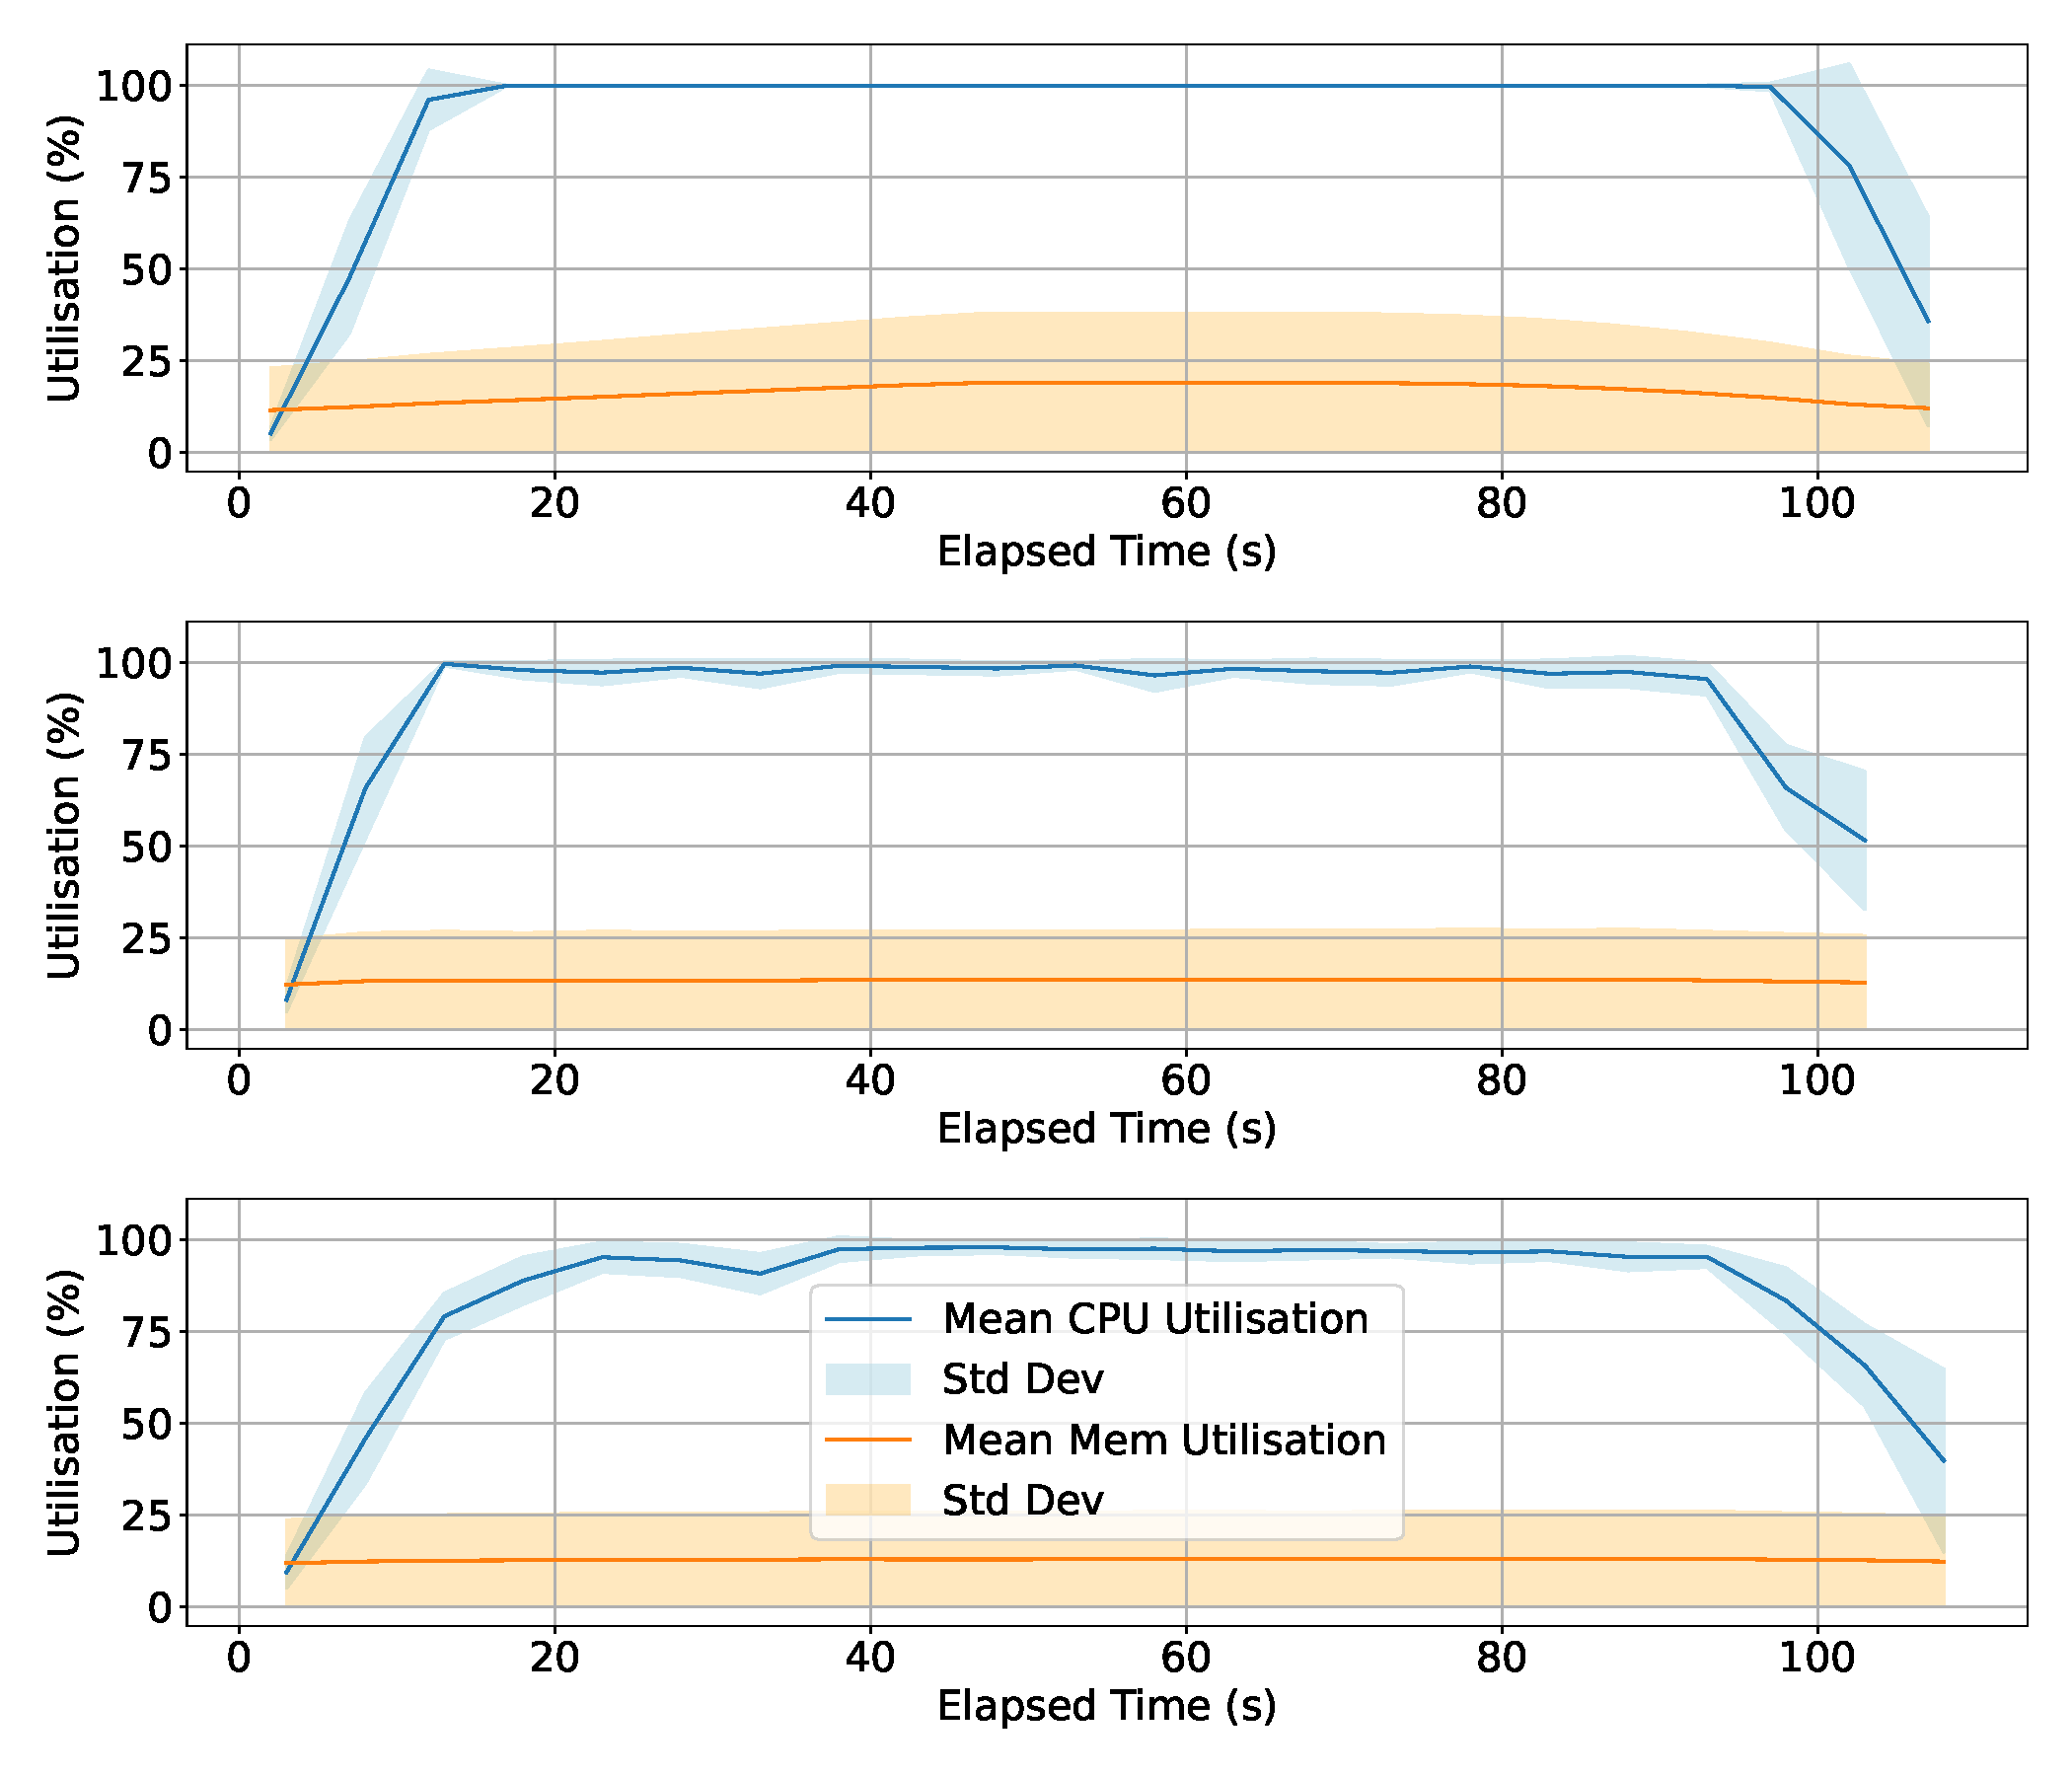
\includegraphics[width=\textwidth]{images/pi-util.pdf}
    \caption{Resource utilisation during the 1000 \texttt{pi-2000} Pod
    Job trace shown in Figure \ref{fig:pi-2000-1000x-pod-running}. Top:
    \texttt{kube-scheduler} (100m). Middle: \texttt{kube-scheduler} (500m).
    Bottom: \textsc{Carico}}
    \label{fig:pi-2000-1000x-pod-util}
\end{figure}

Figure \ref{fig:pi-2000-1000x-pod-util} illustrates the resource utilisation
during the traces of a CPU-focused Job. \texttt{kube-scheduler} achieves
$\approx100$\% CPU utilisation with both 100 and 500 milliCPU requests.
Although, \textsc{Carico} takes a more than twice as long to reach $\geq 95$\%,
it achieves consistently high CPU utilisation.

\begin{figure}[ht!]
    \centering
    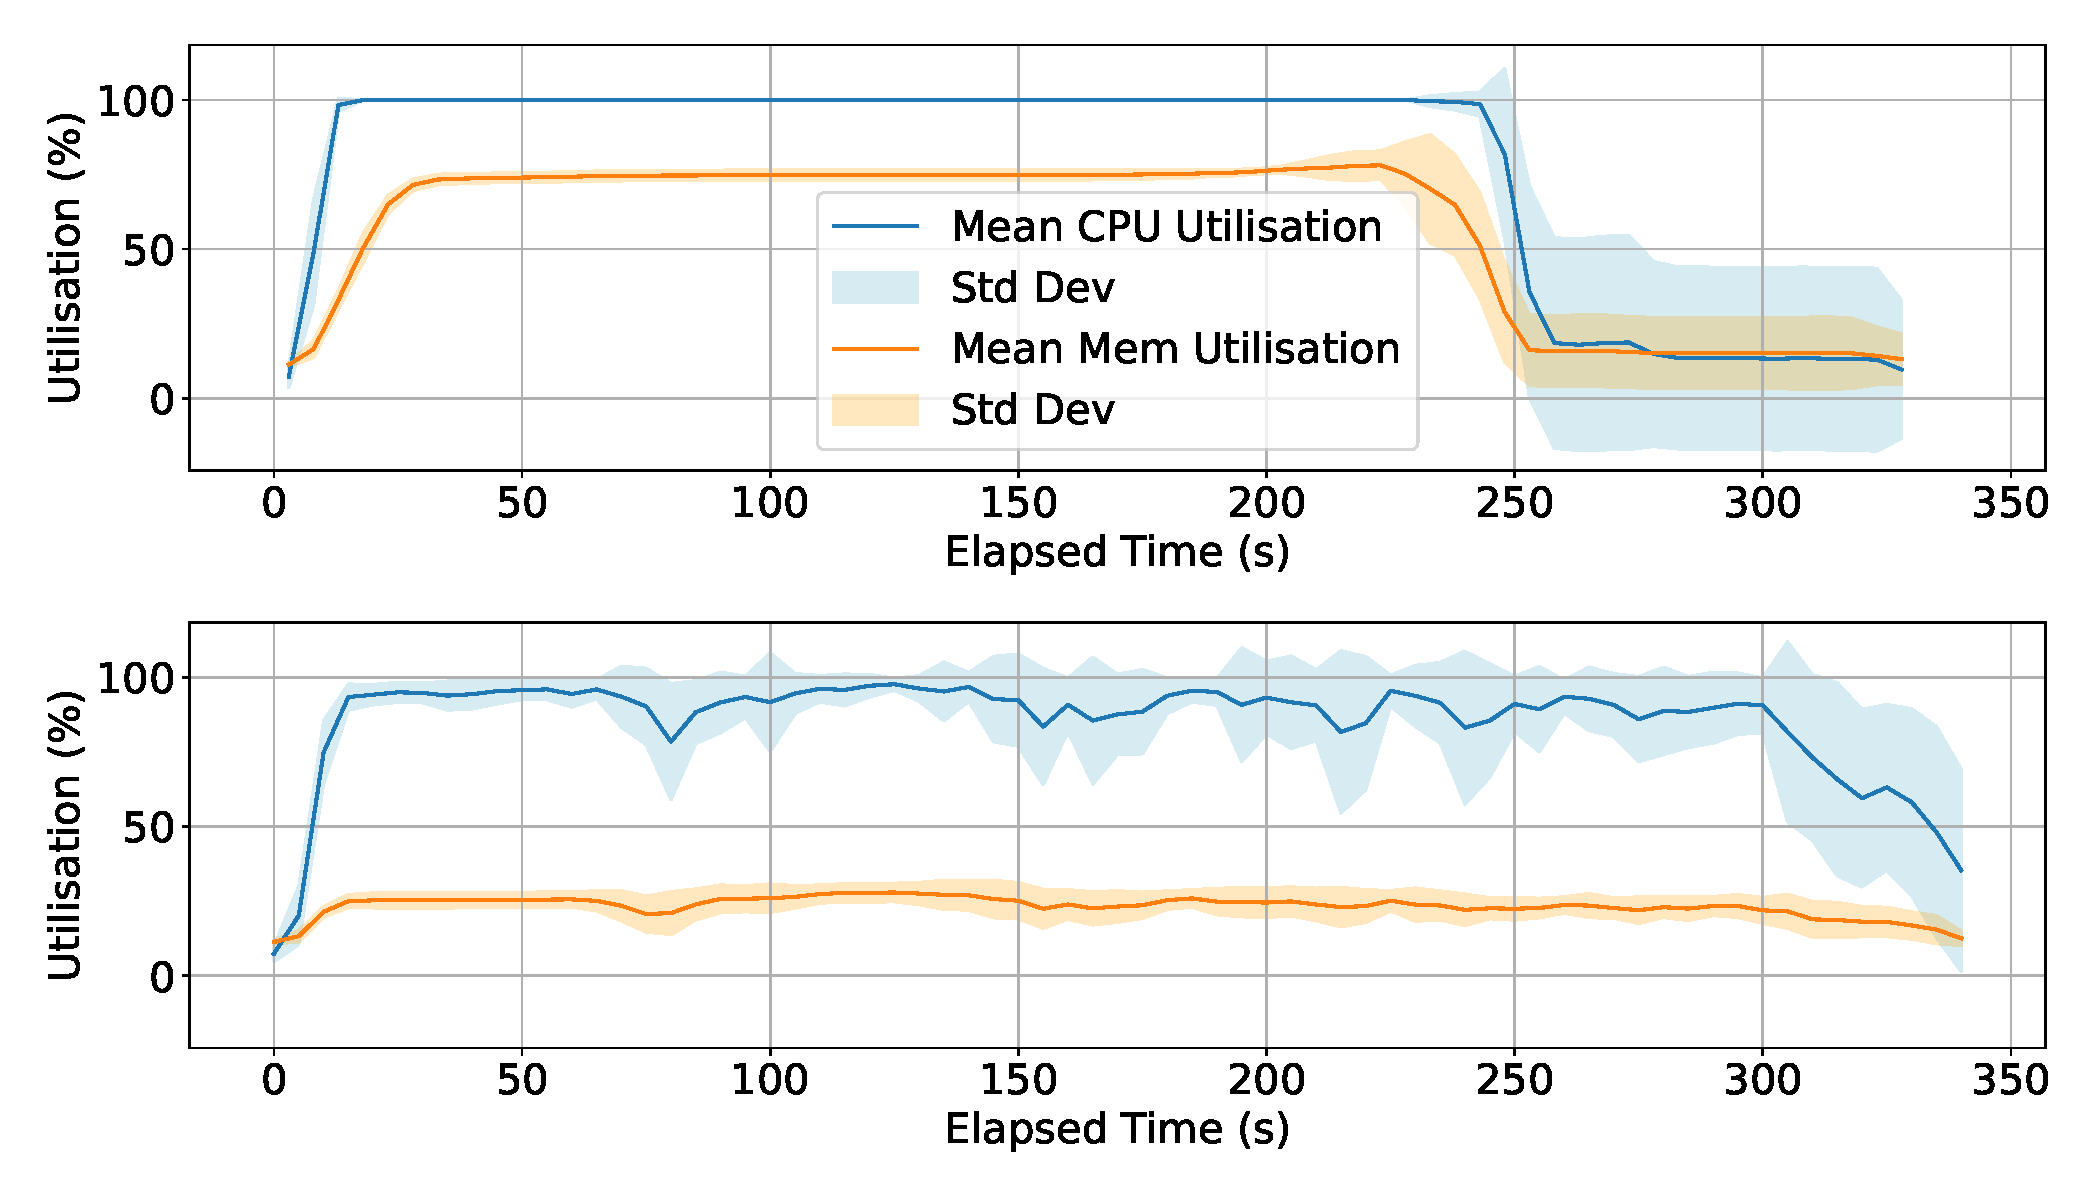
\includegraphics[width=\textwidth]{images/ml-util.pdf}
    \caption{Resource utilisation during the 200 \texttt{sklearn} Pod
    Job trace shown in Figure \ref{fig:ml-pod-running}. Top:
    \texttt{kube-scheduler} (750Mi). Bottom: \textsc{Carico}}
    \label{fig:ml-util}
\end{figure}

Figure \ref{fig:ml-util} presents the resource utilisation during the execution
memory-focused Job. However, the measured resource usage indicates that the CPU
still reaches full capacity before memory. While \texttt{kube-scheduler} still
achieves 100\% CPU utilisation and a high memory utilisation, \textsc{Carico}
results in lower resource utilisation across the cluster. As \textsc{Carico} Pods
predict a high Per-Pod-Cost, a Node's resource usage must drop significantly
before another Pod can be scheduled, resulting in lower resource usage. In
addition, the resulting low Pod-Capacity means that any small variations can
result in a large variance in resource usage.

% While \textsc{Carico} again
% achieves high CPU utilisation, it fails to fully utilise memory. This indicates
% that even with \texttt{sklearn}'s significantly large memory footprint, CPU
% still became the bottleneck resource. As a result, Nodes would limit capacity
% before fully utilising memory. Contrastingly, as \textsc{kube-scheduler} does
% not use live-telemetry, it is able to pack enough \texttt{sklearn} pods to
% achieve a higher memory utilisation. However, this trace also highlights
% problems caused by \texttt{kube-scheduler}'s greedy bin-packing.
% Figure~\ref{fig:ml-pod-running} from Section~\ref{sec:eval-pod-completion}
% painted the scenario in which \texttt{kube-scheduler} results in a mostly idle
% cluster waiting for a small number of machines to finish executing the remaining
% Pods. We can observe this impact on resource utilisation, as during the last
% minute of the Job's execution, the clusters average CPU and memory utilisation
% is around $\approx 10$\%.
%
\section{Workload Heterogeneity}
\label{sec:eval-hetero}
To investigate how \textsc{Carico} handles workloads with different
characteristics, I executed both the \texttt{pi-2000} and \texttt{sklearn} Jobs.

\textbf{Throughput}\\
\begin{figure}[ht!]
    \centering
    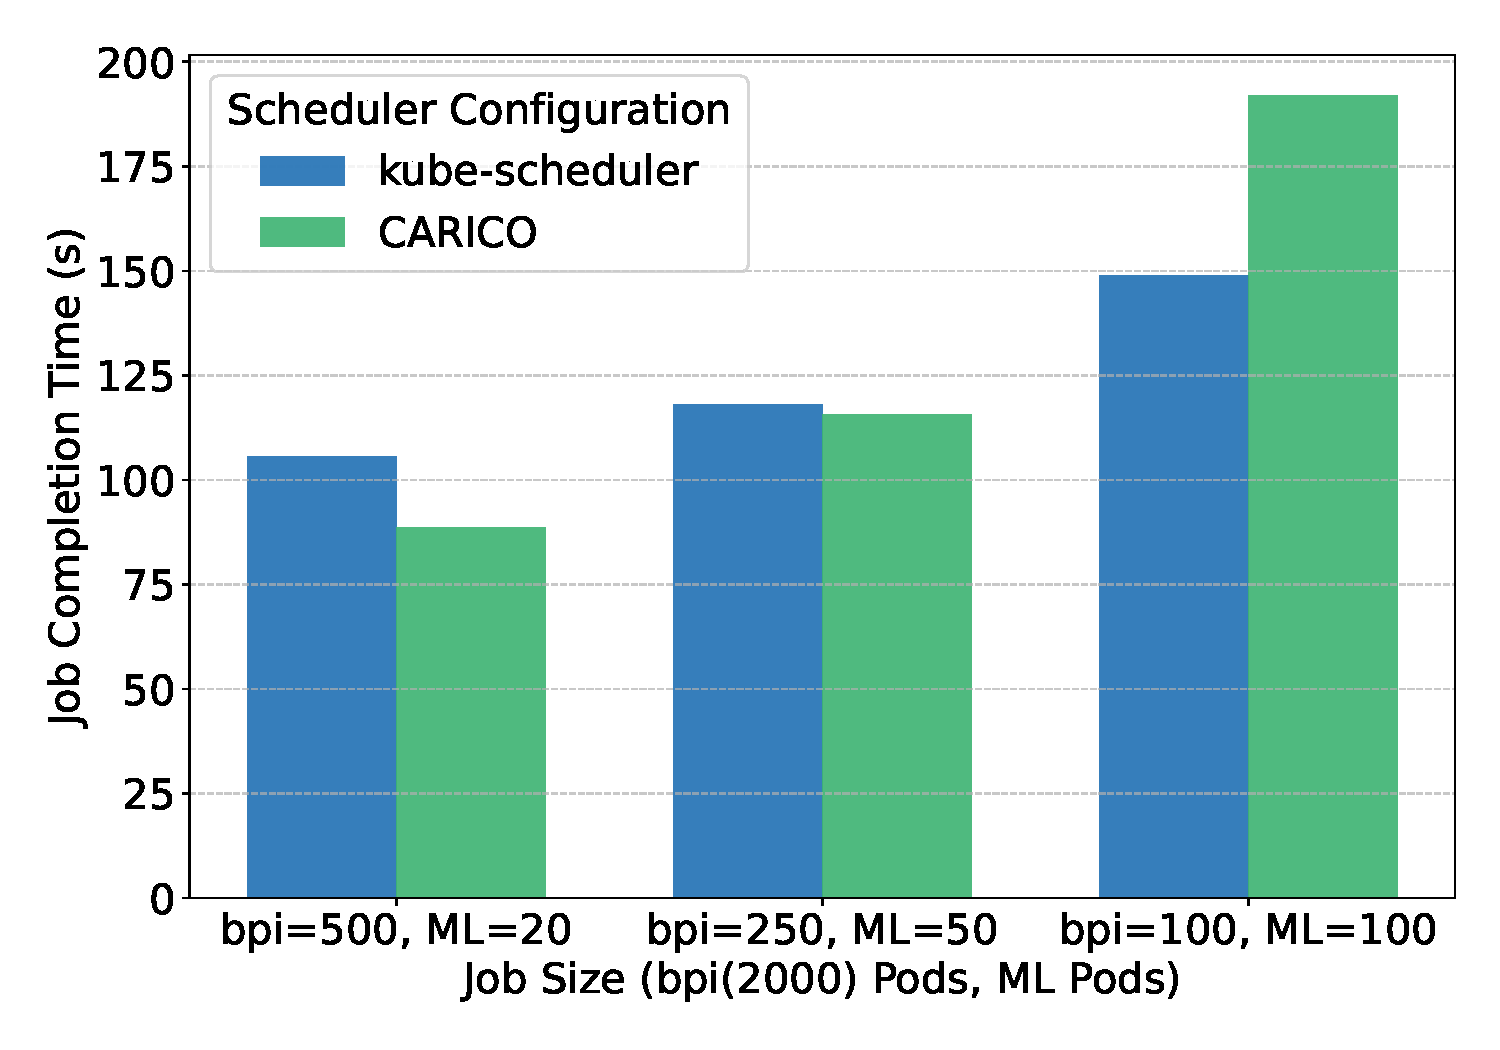
\includegraphics[width=\textwidth]{images/mixed-job-completion.pdf}
    \caption{The Job Completion of multi-resource Job deployments with different Pod
    counts. For the default scheduler, \texttt{pi-2000} Pods request 100
    milliCPUs and \texttt{sklearn} Pods requested 200 milliCPUs and 750Mi of
    memory.}
    \label{fig:mixed-throughput}
\end{figure}

Figure \ref{fig:mixed-throughput} demonstrates that \textsc{Carico} achieve
lower JCT when executing a majority of Pods execute \texttt{pi-2000}.
This indicates \textsc{Carico} is better at handling the interference of many
short Pods on longer running workloads. However, with a smaller \texttt{pi-2000}
Job, the interferences of these Pods is insignificant and JCTs represent those
from running only an \texttt{sklearn} Job. This suggests \textsc{Carico}
continues to exhibit comparable JCT to \texttt{kube-scheduler} when running
heterogeneous workloads.

% \begin{table}[ht!]
% \centering
    % \begin{tabular}{|l|c|c|c|}
    % \hline
    % \textbf{Scheduler} & \multicolumn{2}{c|}{\textbf{Job Size}} &
        % \textbf{Job Completion (s)} \\ \cline{2-3}
        % &  \texttt{bpi(2000)} & \texttt{ML} & \\
    % \hline
        % \texttt{kube-scheduler} & 500 & 20 & 105.7 $\pm$ 10.6 \\
        % \textsc{Carico} & 500 & 20 & 88.7 $\pm$ 2.5 \\
        % \texttt{kube-scheduler} & 250 & 50 & 118 $\pm$ 4.58 \\
        % \textsc{Carico} & 250 & 50 & 115.7 $\pm$ 0.58 \\
        % \texttt{kube-scheduler} & 100 & 100 & 149 $\pm$ 0.0 \\
        % \textsc{Carico} & 100 & 100 & 192 $\pm$ 4.0 \\
    % \hline
    % \end{tabular}
    % \caption{Job Completion of multi-resource Job deployments with different Pod
    % counts. For the default scheduler, \texttt{bpi(2000)} Pods requested 100
    % milliseconds of CPU and ML Pods requested 200 milliseconds CPU and 750Mi of
    % memory}
    % \label{tab:mixed-throughput}
% \end{table}

\textbf{Pod Completions}\\
\begin{table}[ht!]
\centering
    \begin{tabular}{|l|c|c|c|c|c|c|c|c|}
    \hline
        \bfseries Scheduler & \bfseries Job & \bfseries Mean & \bfseries Std. &
        \bfseries Min. & \bfseries 25\% & \bfseries Median & \bfseries 75\% & \bfseries Max. \\
    \hline
        \texttt{kube-scheduler} & \texttt{pi-2000} & 28.78 & 7.52 & 7.00 & 27.00 & 30.00 & 33.00 & 45.00 \\
        \texttt{kube-scheduler} & \texttt{sklearn} & 65.25 & 10.53 & 49.00 & 58.25 & 64.00 & 75.25 & 82.00 \\
        \textsc{Carico} & \texttt{pi-2000} & 7.40 & 1.14 & 5.00 & 7.00 & 7.00 & 8.00 & 11.0 \\
        \textsc{Carico} & \texttt{sklearn} & 34.50 & 7.39 & 22.00 & 27.50 & 36.00 & 40.25 & 44.00 \\
    \hline
    \end{tabular}
    \caption{PCT of a trace when concurrently executing a 500 Pod \texttt{pi-2000}
    Job and a 20 Pod \texttt{sklearn} Job.}
    \label{tab:mixed-pod-completions}
\end{table}

Table \ref{tab:mixed-pod-completions} demonstrates that \textsc{Carico}
continues to achieve significantly tighter and lower PCT distributions than
\texttt{kube-scheduler}; achieves $\approx 7 \times$ lower mean and variance with
\texttt{pi-2000} PCTs.

% TODO: SHOULD I ONLY INVESTIGATE WORKLOADS WE HAVE SEEN BEFORE SO THAT I CAN
% COMPARE THE CHANGE IN DISTRIBUTION

\begin{figure}[ht!]
    \centering
    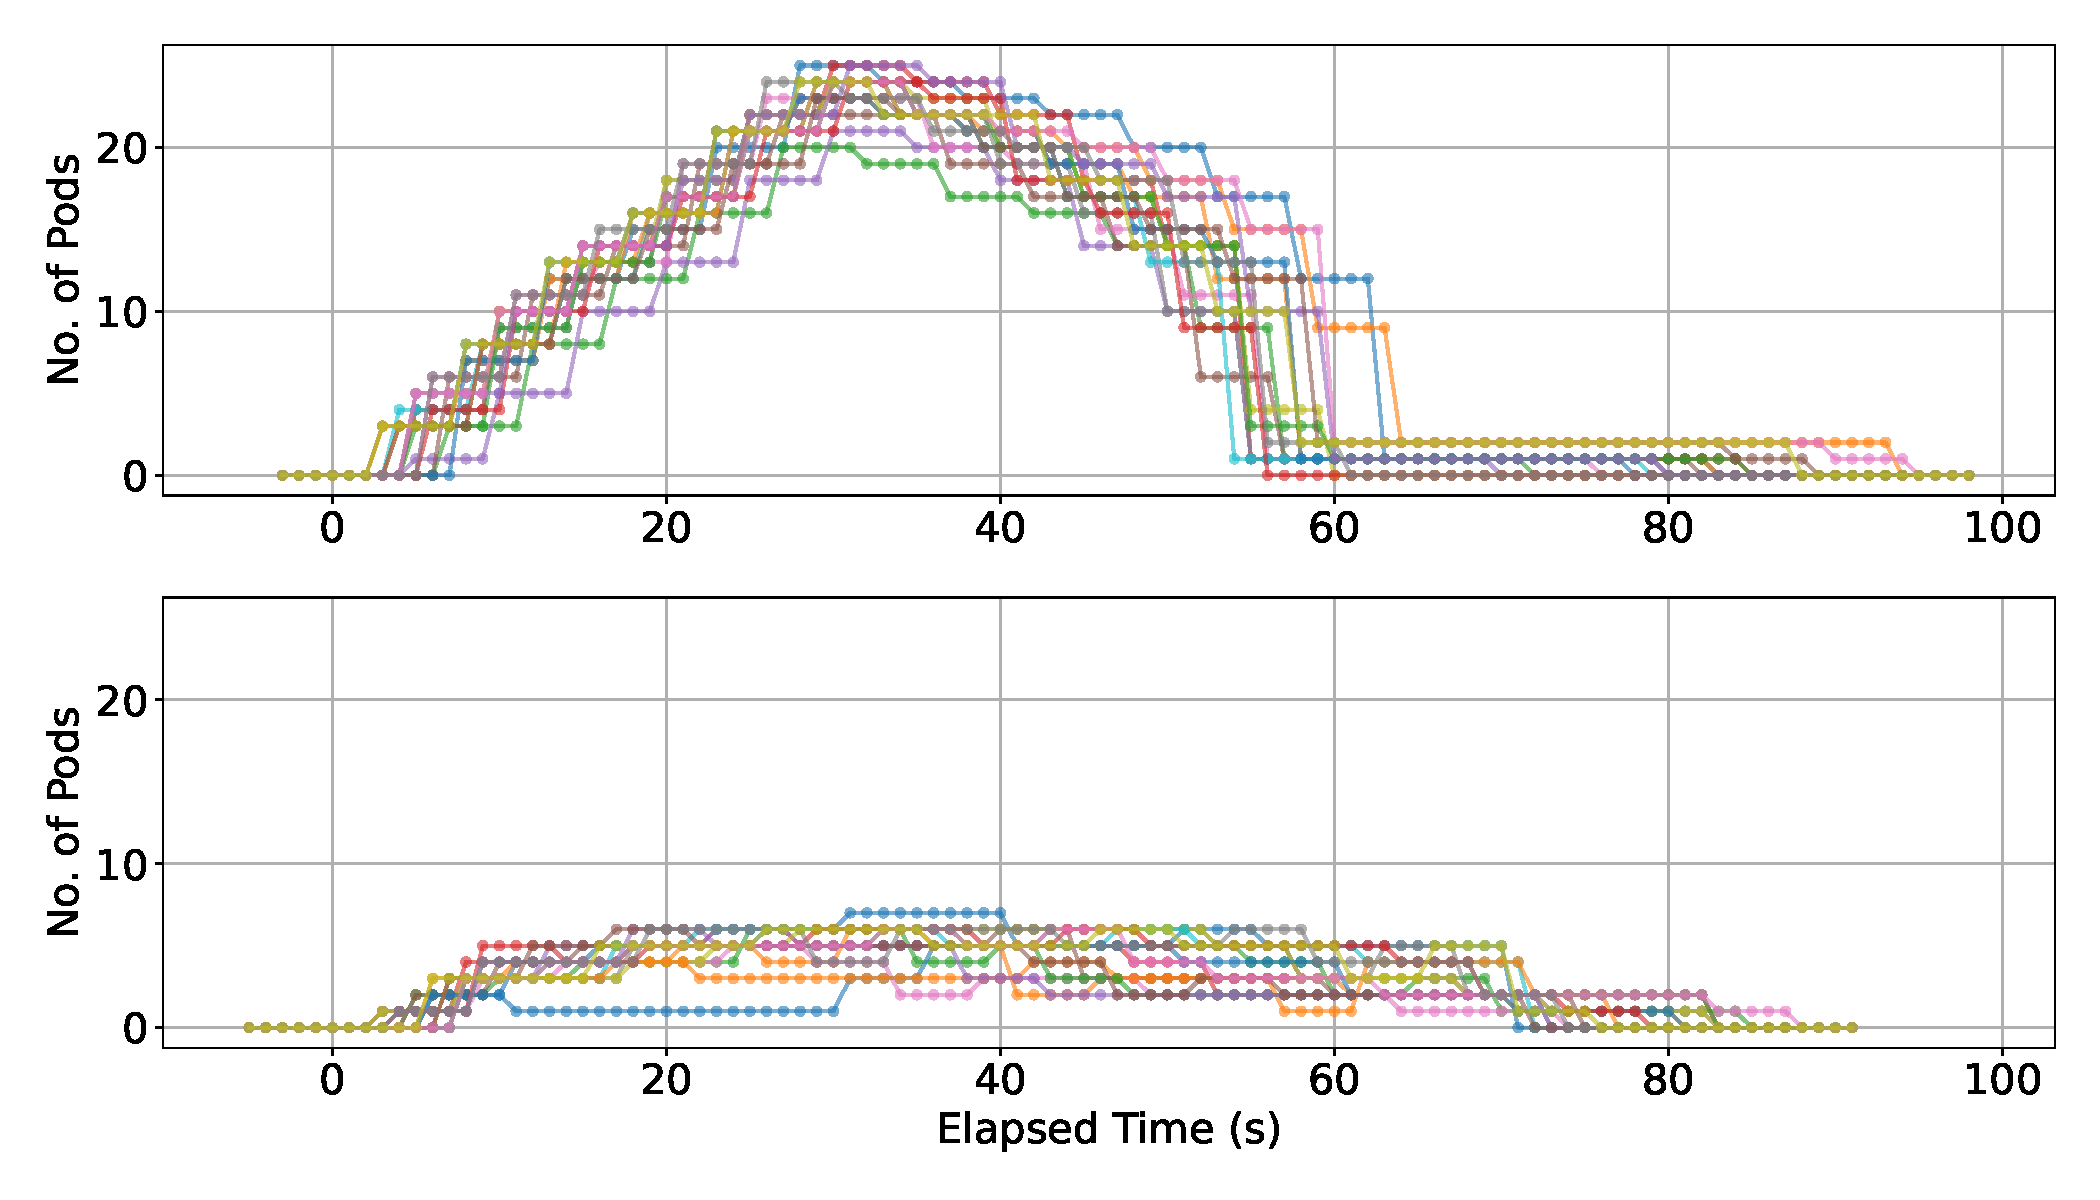
\includegraphics[width=\textwidth]{images/mixed-running-pods.pdf}
    \caption{The number of Pods running on a Node when executing concurrently a
    500 Pod \texttt{pi-2000} Job and a 20 Pod \texttt{sklearn} Job. Top:
    \texttt{kube-scheduler}. Bottom: \textsc{Carico}}
    \label{fig:mixed-pod-running}
\end{figure}

Further investigation into the number of Pods running on each Node, depicted in
Figure \ref{fig:mixed-pod-running}, shows how \textsc{Carico} achieves a
consistent number of running Pods throughout the job, while with
\texttt{kube-scheduler} the number of running Pods varied from 25 Pods to less
than 3 Pods.

\textbf{Resource Utilisation}\\
\begin{figure}[ht!]
    \centering
    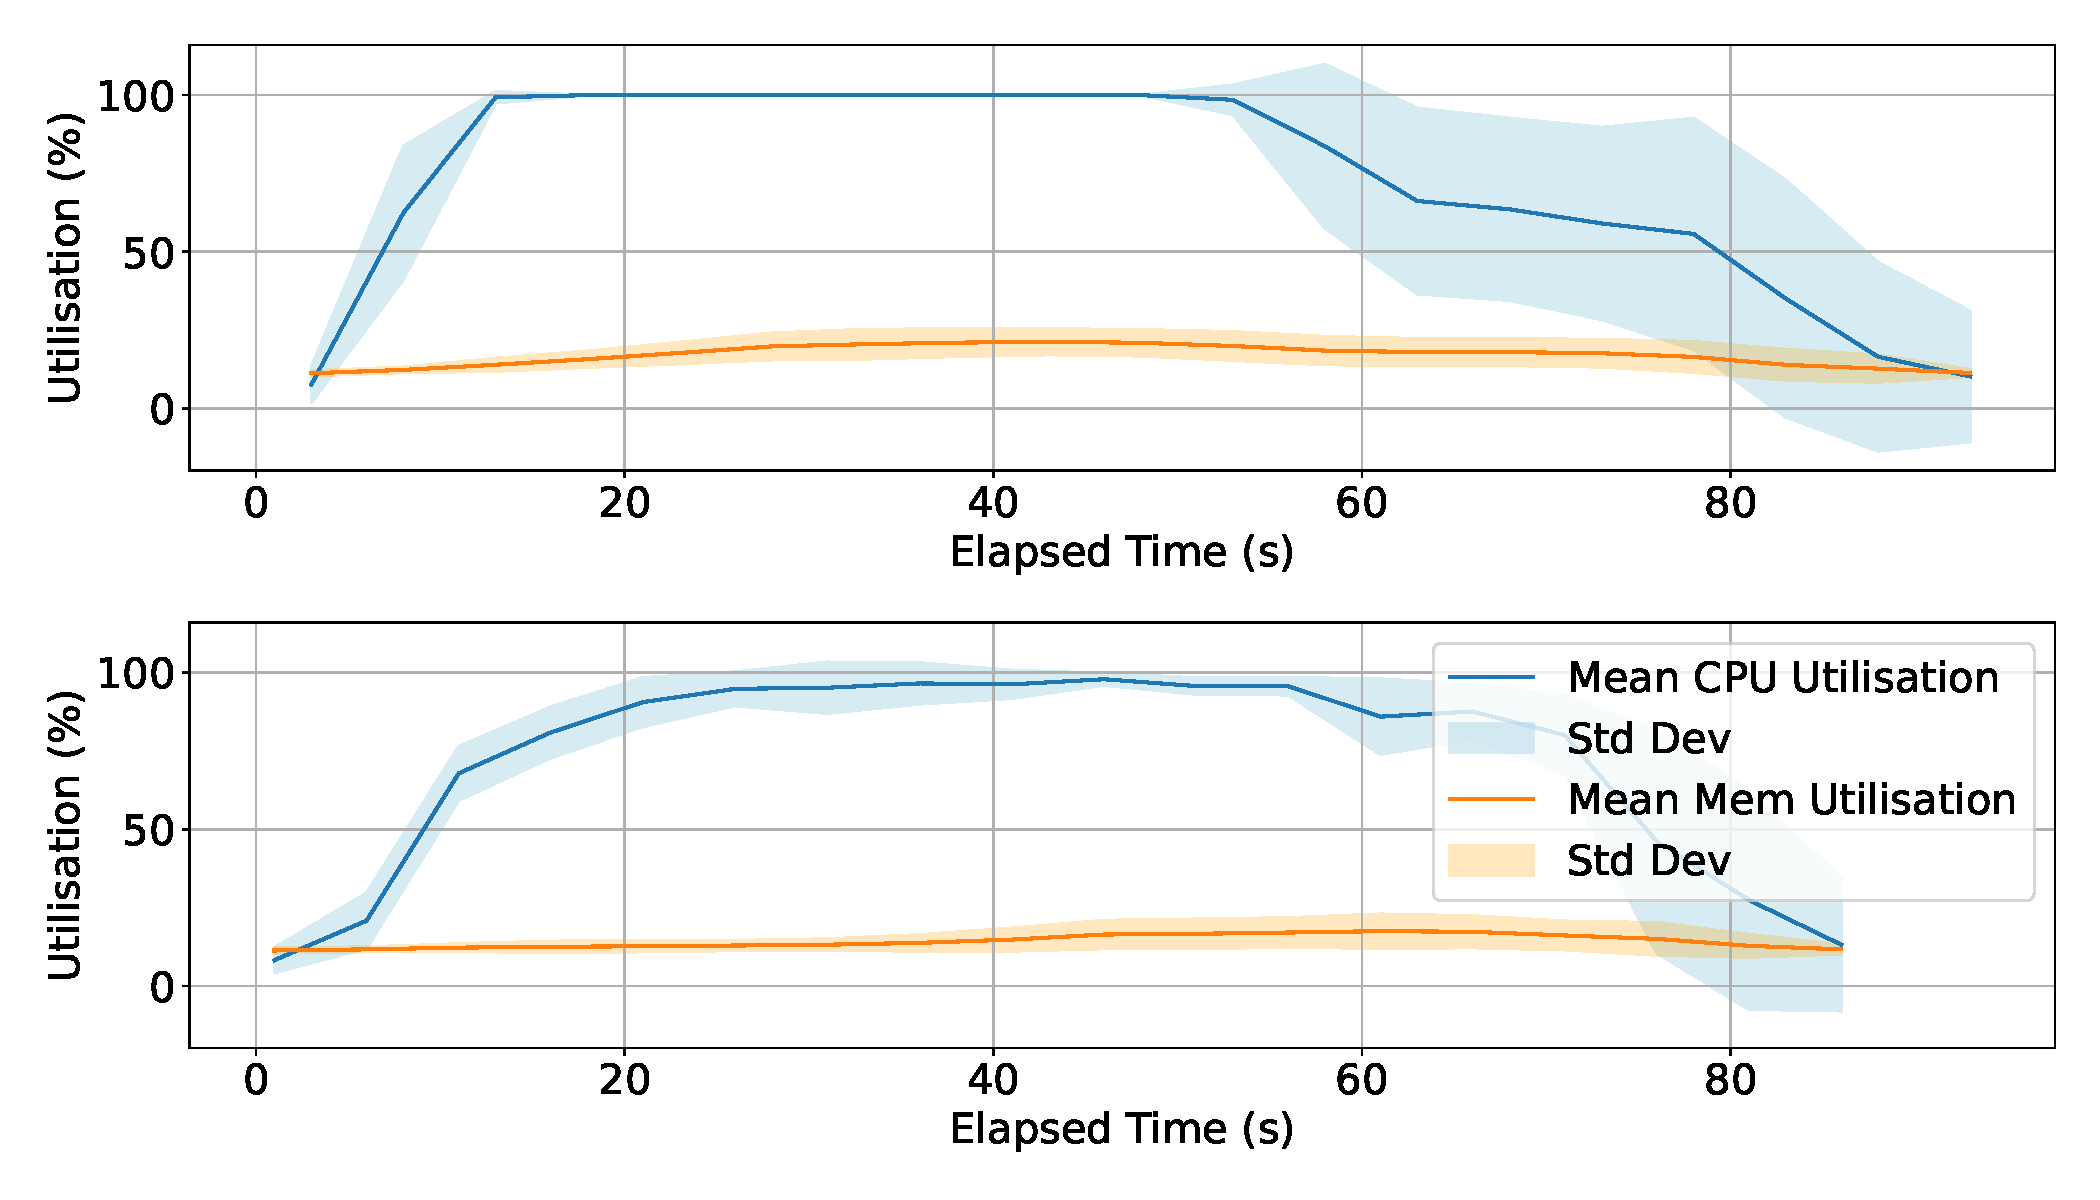
\includegraphics[width=\textwidth]{images/mixed-util.pdf}
    \caption{Resource utilisation during a trace of executing concurrently a 500
    Pod \texttt{pi-2000} Job and a 20 Pod \texttt{sklearn} Job.Top:
    \texttt{kube-scheduler}. Bottom: \textsc{Carico}}
    \label{fig:mixed-util}
\end{figure}

Figure \ref{fig:mixed-util} demonstrates how \textsc{Carico} achieves a resource
utilisation similar to \texttt{kube-scheduler} under a heterogeneous workload.
Interestingly, it achieves a more consistent resource utilisation across the
entire Jobs runtime. This is likely due to \textsc{Carico} achieving a more
balanced and consistent running Pod count (shown in Figure
\ref{fig:mixed-pod-running}).

\textsc{Carico} continues to demonstrate comparable scheduling performance to
\texttt{kube-scheduler}, crucially without relying on resource requests.

\section{Workload Isolation}
\label{sec:eval-isolation}
This experiment use a server Pod running on a worker Node and a separate polling
Pod which periodically sends HTTP GET requests measure the response latency. We
can then measure the impact \textsc{Carico} and \texttt{kube-scheduler} have on
the response latency when they each schedule a large Job.

\begin{table}[h!]
\centering
    \begin{tabular}{|l|c|c|c|c|c|c|}
    \hline
    \textbf{Scenario} & \multicolumn{6}{c|}{\textbf{Response Latency (ms)}} \\
    \cline{2-7}
    & \textbf{Min} & \textbf{Med} & \textbf{P90} & \textbf{P95} & \textbf{P99} & \textbf{Max} \\
    \hline
    Pristine Conditions & 0.99 & 3.04 & 3.78 & 4.00 & 4.47 & 8.32 \\
    \texttt{kube-scheduler} Scheduler & 1.07 & 10.06 & 18.61 & 22.28 & 28.82 & 54.49\\
    \textsc{Carico}  & 1.00 & 2.48 & 6.09 & 7.82 & 10.53 & 17.39\\
    \hline
    \end{tabular}
    \caption{The distribution of a servers response latency when different
    schedulers allocate a 1000 \texttt{pi-2000} Pod Job across the cluster. Pods
    request 100 milliCPU.}
    \label{tab:impacted-latency}
\end{table}

Table \ref{tab:impacted-latency} contains these results and demonstrates that
\texttt{kube-scheduler} significantly shift the response latency distribution,
almost tripling the median and a $\approx \times 7$ larger tail latency.
However, \textsc{Carico} achieves a lower median and only a $\approx \times2$
larger tail latency.

\section{\textsc{Carico} Overhead}
\label{sec:eval-overhead}
Measuring the overhead from the \textsc{Carico} Pods is difficult as its
behaviour changes as Pods arrive or complete. To achieve a holistic measure of
its overhead, we compare the JCT with and without deploying
the \textsc{Carico} Pods. This method considers the additional processing
overhead from event listeners and signal processing techniques, like Kalman
Filters.

\begin{table}[ht!]
\centering
    \begin{tabular}{|c|c|}
    \hline
    \textbf{Number of Pods} & \textbf{\% Difference in JCT} \\
    \hline
        100 & -2.33 $\pm$ 3.29 \\
        250 & -1.19 $\pm$ 2.44 \\
        500 & 4.84  $\pm$ 1.25 \\
        750 & 1.69  $\pm$ 0.42 \\
        1000 & 2.27  $\pm$ 0.66 \\
    \hline
    \end{tabular}
    \label{tab:overhead}
    \caption{The \% difference in JCT when executing 1000 a \texttt{pi-2000}
    Pod Job with and without \textsc{Carico} Pods. Pods are scheduled by
    \texttt{kube-scheduler} and request 100 milliCPU.}
\end{table}

Table \ref{tab:overhead} presents the relative change in JCT defined as:
\[
\frac{\text{JCT}_{\text{with Carico}} - \text{JCT}_{\text{without
Carico}}}{\text{JCT}_{\text{without Carico}}}
\]
Smaller Jobs reported a decrease
in JCT, however the large variance indicates these are likely a product of
noise. The smaller variance with larger Jobs suggests more stable and thus
representative results. Thus, we can ascertain that \textsc{Carico} has
$\approx$ 2\% overhead.

\section{Limitations}

Firstly, \textsc{Carico} is a telemetry-based scheduler and thus relies on accurate
telemetry that is able to accurately capture a Node's true limit, after which
over-contention results in degraded performance. During this dissertation, we
have observed how this is not guaranteed. VMs, like those I used in my
evaluation, only have access to a simulated hardware provided by the underlying
hypervisor. As a result, symptoms of over-contention, such as the overhead from
CPU or cache thrashing, are not observed when a VM reports high CPU utilisation.
This supported by Figure \ref{fig:podcount-util-pressure}: the Job Completion
time per Pod when executing a Job on a single Node, continued to decrease even
after the Node reported full CPU pressure. Consequently, \textsc{Carico}
allocates fewer Pods to Nodes reducing Job completion.

Secondly, \textsc{Carico} can only learn about Pod workloads once they have
already been scheduled and observed. This can limit performance, as
\textsc{Carico} is unable to discern new Pods with potentially complementary directions
of resource usage from those it has already observed. Conversely, a
high-intensity workload may be submitted after a low-intensity one, and
\textsc{Carico}'s recent low Per-Pod-Cost estimate could result in a over-eager
Nodes accepting too many high-intensity workloads before \textsc{Carico} has
time to detect the new resource usage. This situation could then cause
performance degradation or even the termination of Pods. \textsc{Carico}
attempts to mitigate this by having the Per-Pod-Cost slowly increase when there
are no Pods running, however, this has a limited impact for workloads that
arrive in quick succession.
